\input{style/settings}
\input{style/short_commands}
\pagestyle{fancy}
\fancyhf{}
\fancyhead[R]{página\;\thepage/\pageref{LastPage}}
\fancyhead[L]{Osvaldo Uriel Calderón Dorantes}
\fancyfoot[L]{Imagenología Biomédica}
\fancyfoot[R]{Facultad de Ciencias, UNAM 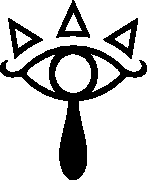
\includegraphics[scale=0.13]{style/Sheikah.pdf}}
\fancypagestyle{plain}{
  \fancyfoot[C]{}
}
\makeatletter
\def\@seccntformat#1{%
  \expandafter\ifx\csname c@#1\endcsname\c@section\else
  \csname the#1\endcsname\quad
  \fi}
\makeatother
%%%%%%%%%%%%%%%%%%%%%%%%%%%%%%%%%%%%%%%%%%%%%%%%%%%%%%%
%%%%%%%%%%%%%%%%%%%%%%%%%%%%%%%%%%%%%%%%%%%%%%%%%%%%%%%%%%%
\begin{document}
\begin{flushleft}
Osvaldo Uriel Calderón Dorantes, \hfill Imagenología Biomédica\\
316005171 \hfill osvaldo13576@ciencias.unam  \\
Facultad de Ciencias\\
\underline{Universidad Nacional Autónoma de México}
\end{flushleft}

\begin{flushright}\vspace{-5mm}

\includegraphics[height=1.5cm]{style/logo.pdf}
\end{flushright}
 
\begin{center}\vspace{-1cm}
\textbf{ \large \customfont{Cuestionario 1\\
Módulo RESONANCIA MAGNÉTICA}}\\
\today
\end{center}
%\medskip\hrule\medskip
%%%%%%%%%%%%%%%%%%%%%%%%%%%%%%%%%%%%%%%%%%%%%%%%
%{\small \textbf{Nota: A las unidades las pondré dentro de corchetes \ec{[\tx{unidad}]} para no confundir entre variables y realizar el análisis dimensional fácilmente.}}
\medskip\hrule\bigskip

\newlength{\strutheight}
\settoheight{\strutheight}{\strut}


\begin{enumerate}
  \item ¿Cuáles son las 4 zonas que conforman un área de Resonancia Magnética?
  
\begin{itemize}
  \item \textbf{Zona 1: Recepción y área de espera.} Es la parte donde se recibe al paciente y su documentación, en esta región no hay campo magnético \ec{\vec{B}=\vec{0}}.
  \item \textbf{Zona 2: Vestimenta y prescripción del paciente.} El paciente es donde el paciente puede almacenar sus pertenencias y se pueden realizar preparativos clínicos, en esta región no hay campo magnético \ec{\vec{B}=\vec{0}}.
  \item \textbf{Zona 3: Estación de tecnólogo de la sala de control de resonancia.} Esta sala de control es donde trabajará el técnico o médico radiólogo para poder adquirir las imágenes, el campo magnético en esta región es \ec{\vec{B}\neq\vec{0}}, aunque no es muy intenso.
  \item \textbf{Zona 4: Sala de Imán.} En esta sala se encuentra el equipo de resonancia magnética y el campo magnético es más intenso. 
\end{itemize}


  \item ¿Qué es un QUENCH?
  
  Es cuando el imán superconductor pierde sus propiedades superconductivas al liberar los criogénicos, entonces el aumento de temperatura hace que el imán pierda esa propiedad. En la sala de imanes existe un botón para QUENCH y debe accionarse solo en caso de emergencia para salvaguardar la integridad del paciente, cuando éste se acciona el criogénico se evapora y se libera fuera del edificio.



  \item Explique qué es la constante giromagnética.
  
La constante giromagnética \ec{\gamma} indica la cual giran los núcleos cuando están dentro de un campo magnético, este valor es característico de cada núcleo y determina la frecuencia de Larmor \ec{\omega} en un campo magnético \ec{B_0} dado. Es decir la frecuencia de Larmor es directamente proporcional a la intensidad del campo magnético siendo la constante giromagnética la constante de proporcionalidad, por ejemplo, para el hidrógeno su valor es \ec{\gamma=42.57\un{MHz\ec{\cdot}T\ec{^{-1}}}}.



  \item ¿Cómo se genera la magnetización neta?
  
La magnetización neta se refiere cuando se tiene la suma total de todos los momentos magnéticos de los átomos de hidrógeno, se genera debido a la propiedad cuántica de los átomos de hidrógeno que es el espín, los cuales en presencia de un campo magnético \ec{\vec{B}_0} hacen que se alineen en dirección al campo magnético y son paralelos (tienen un estado de baja energía) y los que se alinean en dirección opuesta al campo son antiparalelos (estado de alta energía). 






  \item ¿En qué consiste el fenómeno de Resonancia Magnética?
  
Este fenómeno surge cuando el vector de magnetización es perturbado de su orientación en equilibrio. Consiste en la absorción de la radiación electromagnética de los núcleos de un cuerpo cuando está dentro de un campo magnético, entonces se emite una radiación con la misma frecuencia de resonancia la cual depende del campo magnético  y también de las propiedades atómicas del cuerpo. 


\end{enumerate}


%\begin{multicols}{2}
%\small{\bibliographystyle{apalike}
%\bibliography{bib}}
%\end{multicols}



%\ftikz{1.5}{figuras/fig.tikz}{}{fig:x}

\end{document}



